%%%%%%%%%%%%%%%%%%%%%%%%%%%%%%
%%%%%%%% Motivation %%%%%%%%%%
%%%%%%%%%%%%%%%%%%%%%%%%%%%%%%
\chapter{Motivation}

Nowadays machine learning and deep learning have become a distinguished approach for visual
recognition tasks and has achieved great success in this process. However, they seek a large amount of
labeled data to learn. Providing this amount of labeled data not only will bring much effort along but also will occupy a huge size of storage and seek large storage. In
contrast, humans are very good in visual recognition so that, they can learn with one \footnote{This
  is known as one-shot learning in deep learning and represents the scenario when there is one
  instance of each class in training-set to learn.} or few \footnote{This is known as few-shot learning in
  deep learning and represents the scenario when there are just few instances of each class in
  training-set to learn.}
examples. Imagine one kid who can recognize a lion in a picture
after looking a few pictures of lions as an example. We want to simulate and apply this human’s
ability to
the deep learning and make them learn with few examples, with desirable accuracy.
In this bachelor thesis, we concern ourselves with few-shot learning in deep learning. We aim to
learn and train a model when there are few labeled examples obtainable. We approach to generate
artificial examples from a few available labeled examples and enalrge our dataset artificially.
This technique known as data augmentation. These artificial labeled examples aid us to learn better
with more accuracy and prevent overfitting. Data augmentation is our focus in this work to achieve few-shot
learning and prevent overfitting. In this thesis, we will introduce different well-known methods of
data augmentation. The first purpose will be to discover if and how far data augmentation can
improve the learning process and accuracy. The second step will be to compare their accuracy. In
the end, we aim to discover the potential possibility of combining the different methods of data
augmentation to increase accuracy and reduce error-rate and improve the learning process.
We will focus on visual recognition tasks and their classification. Additionally, we will concentrate on the implementation of various methods of data augmentation for convolutional neural networks


%%%%%%%%%%%%%%%%%%%%%%%%%%%%%%
%%%%%%%% Introduction %%%%%%%%
%%%%%%%%%%%%%%%%%%%%%%%%%%%%%%
\chapter{Introduction}

Neural networks can possibly contain multiple non-linear layers and this makes them very expressive models
that can learn very complicated relationships between their inputs and outputs. With even limited
input data, neural networks can discover and learn many relations from the data, however, sometimes the
discovered and learned relations do not exist or just consist of redundant information and
relations. Redudant relation can potentially arise of data-noise or lack of data-generalization. Non
exist relations can potentially emerge from lack of enough data. These phenomena known as
\textit{overffiting} in deep learning. In other words, learning with few labeled examples or noisy
data causes overfitting. Overffiting cause low accuracy and high error-rate. Hence, we approach to propagation of artificial
labeled examples from a few given examples to prevent overfitting and reduce the error rate and increase
the accuracy.

As we mentioned aquiring a huge labeled dataset is expensive and seeks much effort and time. Therefore we aim to generate artificial example from few obtainable labeled examples. In other words, we
augment our data and this strategy is known as data augmentation. There are a few well-known methods for data augmentation. We aim to introduce them in this thesis.  Besides we will implement these
methods to compare their efficiency and capability. These methods are as follow:
\begin{itemize}
  \item \textbf{Label Preserving Transformation} \ref{tit:label-preserving}
  \item \textbf{Elastic Distrotion} \ref{tit:elastic-distrotion}
  \item \textbf{Stroke Warping} \ref{tit:stroke-warping}
  \item \textbf{Bayesian Approach} \ref{tit:bayesian-approach}
\end{itemize}



%%%%%%%%%%%%%%%%%%%%%%%%%%%%%%
%%%%% Data Representation %%%%
%%%%%%%%%%%%%%%%%%%%%%%%%%%%%%
\chapter{Data Representation}
\label{tit:data-representation}
In this chapter, we will briefly introduce the datasets which we use in this work to evaluate the
performance of each data augmentation approach pragmatically. There are mainly $2$ reasons that we
have chosen these datasets. First, they are well-know datasets and there are many researchers on
them and many reported results. Additionally, they are simple enough to learn and append non-complex
classifiers to classify them with desirable accuracy. The second reason is that all these $3$
datasets have $10$ classes with small differences. All of these aids us to have a better and more
realistic benchmark. 

\section{MNIST}
The MNIST dataset (Modified National Institute of Standards and Technology) is a large handwritten
digits dataset, provided by Yann Le Cun, derived from NIST Special Database 19 \cite{NIST}.

The MSNIT dataset consists of $60,000$ train- and $10,000$ test-images and each image is grayscale
with $28 \times 28$ pixels. It has $10$ classes that represent $0-9$ digits and data is fairly
splitted between classes \cite{MNIST_data_reference}. MNIST is one of the most popular datasets for
deep learning because of the not too high complexity and compatibility with almost all deep learning
models. Hence many papers attempted to reach a low error-rate on this dataset. One of them manages
to reduce the error-rate on the MNIST by up to $0.23\%$ \cite{MNIST_best_result_reference}. You can
find the information about the dataset at the table
\ref{dataset_table} and the figure \ref{fig:mnist_dataset_example} shows an example of the dataset.

\begin{figure}
  \centering
  \label{fig:mnist_dataset_example}
  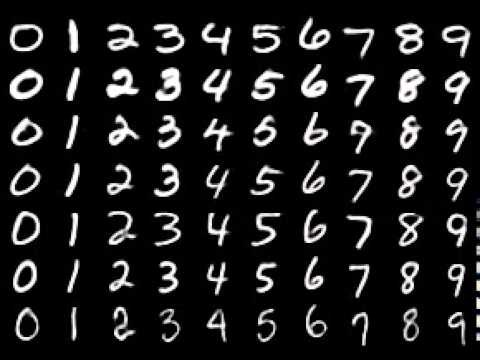
\includegraphics[width=0.5\textwidth]{fig/mnist}
  \caption{7 examples per class of MNIST dataset, merged in one image \cite{MNIST_dataset_example}}
\end{figure}


\section{Fashsion-MNIST}
The Fashsion-MNIST is a dataset of Zalando's \footnote{\url{https://jobs.zalando.com/de/tech/}}
article images provided by Han Xiao et al. \cite{Fashion_MNIST_reference} for benchmarking machine learning algorithms. 

The Fashsion-MNIST dataset as same as MNIST dataset consists of $60,000$ train- and $10,000$ test-images and each image is grayscale
with $28 \times 28$ pixels. It has $10$ classes ([T-Shirt, Trouser, Pullover, Dress, Coat,
Sandal, Shirt, Sneaker, Bag, Ankle Boot]) and the data is fairly
splitted between these classes. One the best reported accuracy on this dataset with convolutional neural
network \footnote{\url{https://github.com/zalandoresearch/fashion-mnist\#benchmark/}} is $91.90\%$. You can
find the information about the dataset at the table
\ref{dataset_table} and the figure \ref{fig:fashion_mnist_dataset_example} shows an example of the dataset.


\begin{figure}
  \centering
  \label{fig:fashion_mnist_dataset_example}
  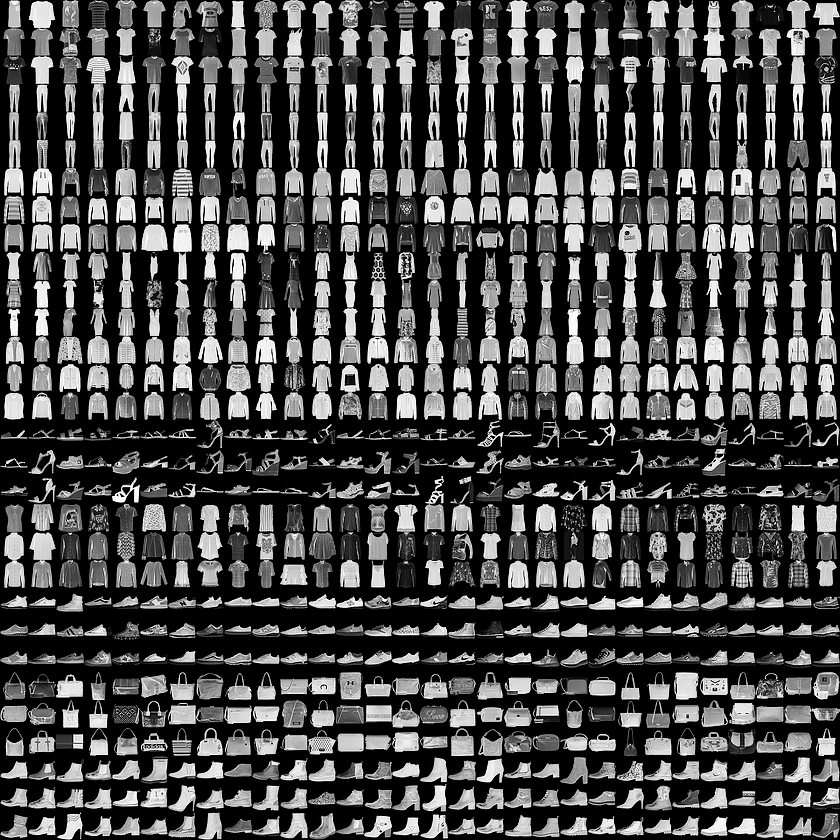
\includegraphics[width=0.5\textwidth]{fig/fashion-mnist-dataset_example}
  \caption{Examples of Fashion-MNIST dataset, merged in one image}
\end{figure}

\section{CIFAR-10}
The CIFAR-10 (Canadian Institute for Advanced Research)
, collected by Alex Krizhevsky, Vinod Nair, and Geoffrey Hinton is a subset from 80 million tiny
images dataset \cite{CIFAR-10_origin_dataset}.

The dataset consists of $60,000$  RGB with $32 \times 32$ pixels images, which are divided to the $50,000$ train and $10,000$ test datasets. As the name makes it clear the CIFAR-10 contains 10 classes ([plane, car, bird, cat, deer, dog, frog, horse, ship, truck]) \cite{CIFAR-10_dataset_reference}.
One of the lowest reported error-rate with a convolutional neural network managed to achieve $2.56\%$ \cite{CIFAR-10_best_result_reference}.  You can
find the information about the dataset at the table
\ref{dataset_table} and the figure \ref{fig:cifar-10_dataset_example} shows an example of the dataset.

\begin{figure}
  \centering
  \label{fig:cifar-10_dataset_example}
  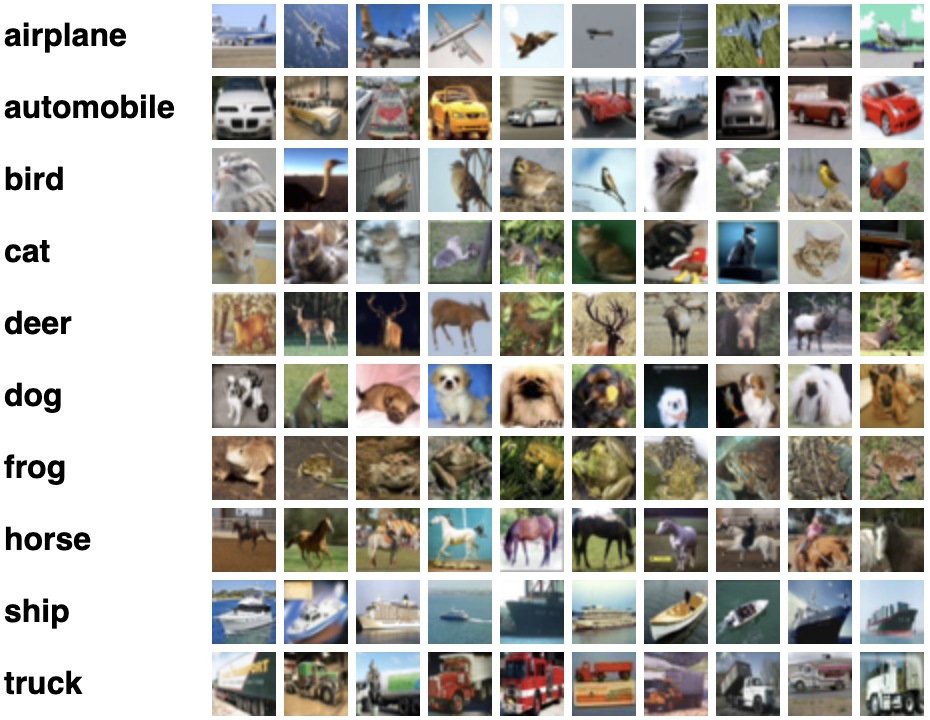
\includegraphics[width=0.5\textwidth]{fig/cifar-10}
  \caption{10 examples per class of CIFAR-10 dataset, merged in one image \cite{CIFAR-10_dataset_reference}}
\end{figure}




\begin{table}[]
  \label{dataset_table}
  \begin{tabular}{
      l |
      c
      c
      c
      c
      c}
    \hline
    {\textbf{Dataset}}        & \multicolumn{1}{l}{{\textbf{NO. Classes}}} & \multicolumn{1}{l}{{\textbf{NO. Train}}} & \multicolumn{1}{r}{{\textbf{NO. Test}}} & \multicolumn{1}{l}{{\textbf{Size (pixel)}}} & \multicolumn{1}{l}{{\textbf{NO. Channel}}} \\ \hline
    {\textbf{MNIST}}          & 10                                         & 60,000
    & 10,000                                  & $28\times28$                                & 1
    (Grayscale)                              \\
    {\textbf{Fashsion-MNIST}} & 10                                         & 60,000
    &10,000                                         &  $28\times28$
    &  1 (Grayscale)                                         \\
    {\textbf{CIFAR-10}}       & 10                                         & 50,000
    & 10,000                                  & $32\times32$                                & 3
    (RGB)                                         \\ \hline
  \end{tabular}
  \caption{Structure of datasets.}
\end{table}


%%%%%%%%%%%%%%%%%%%%%%%%%%%%%%
%%%%% Neural Network %%%%%%%%%
%%%%%%%%%%%%%%%%%%%%%%%%%%%%%%
\chapter{Preliminaries}
\section{Introduction}
\section{Convolutional Neural Network}
\section{Overffiting}


%%%%%%%%%%%%%%%%%%%%%%%%%%%%%%
%%%%%%% Data Augmentaion %%%%%
%%%%%%%%%%%%%%%%%%%%%%%%%%%%%%
\chapter{Data Augmentaion}

In this chapter, we will introduce a few noteworthy related works in this field which are mainly consist of $2$ approaches and several techniques.
In what follows, we solely focus on image data.  While some techniques might be applicable to other
types of data as well, we shall explore them when used on image datasets.

As the name clears itself, we looking for enlarging datasets artificially and generate synthetic
data based on the obtainable few samples to increase the accuracy of the prediction.

\section{Label Preserving Transformations}
\label{tit:label-preserving}
When training neural networks, label preserving transformations are a commonly used approach with classes of
techniques for enlarging datasets by generating generic data. The advantage of using this approach
and its techniques, when available, is twofold. The first benefit is the low space complexity of these
methods since one does not necessarily need to save the generated data on storage. Also, these
transformations are usually of relatively smaller time complexity compared to other approaches,
which makes them desirable in many instances in practice.

As the name may suggest, the ultimate goal when using these techniques is to generate synthetic data points after applying a set of suitable transformations to a real data point.

\subsection{Image Translations}
Image translations is one of the simplest and meanwhile applicable well-known technique of the lable
preserving transformations approach. As the research by Krizhevsky et al.
\cite{image_translation_paper} proposes, we extract
image translations and their horizontal reflections to generate the synthetic data and augment the
dataset. Image translation consists of extracting patches that are smaller in size than original
images. Given a single channel (grayscale) $n \times n$ image and a translation patch of the size
$m$ for some $m<n$, one can produce $(n-m+1) \times (n-m+1) $ synthetic instances of the datapoint. Also, taking
the horizontal reflections of each newly generated data point into account, one can enlarge the
dataset by a factor of 2, therefore finally dataset can be enlarged by factor: $$2\times(n-m+1)\times(n-m+1)$$ 

Figure \ref{fig:label-preserving-trasformation} is an illustration of the translations and horizontal
reflections of a $4 \times 4$ image, using all
possible patches of the size $3 \times 3$, which results in $8$ new data points.

At test (prediction) time, the method extracts the patches with the same size ($m < n$), however this time the
patches will be extracted from 4 corners and center of the test image. The network predicts on these
five patches and their horizontal reflections (10 patches altogether). In the end, the average
on the softmax layer will be determined the final prediction.

\begin{figure}
  \centering
  \label{fig:label-preserving-trasformation}
  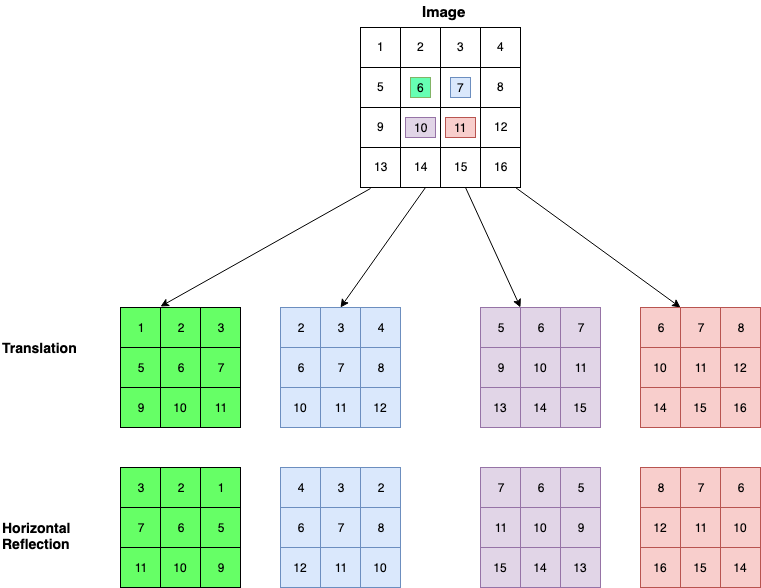
\includegraphics[width=1\textwidth]{fig/label-preserving-transformation}
  \caption{An example of single channel image with size of $4\times4$ with its translations with size of $3\times3$ patches and their horizontal reflections. The numbers determinate the pixels intensity}
\end{figure}


\subsection{Elastic Distortion}
\label{tit:elastic-distrotion}
Another well-known technique for data augmentation is elastic distortion. Quite similar to the image
translations, the ultimate goal is to generate synthetic data set from a single data point. However, instead of
taking patches which are smaller than the original image, the synthetically produced data points are
of the same size as the original image as proposed by \cite{elastic_distortion_paper} . This is done by moving pixels and modifying pixel intensity
according to both their former and new position.  To this end, a few interpolation schemes such as
the nearest neighbor, bicubic, spline, and bilinear are available. Due to their practical
effectiveness and simplicity, we use the bilinear interpolation scheme in this work, which we
discuss in detail below. 

Let $\alpha \in \mathbb{R}$, and let $\Delta x(x,  y) = \alpha x$ and $\Delta y(x,  y) = \alpha y$
denote the horizontal and the vertical displacement of a point $(x, y)$ of an image respectively.
Since the scaling parameter $\alpha$ could take a non-integer value, the interpolation task is
necessary for adjusting the intensity of pixels. Utilizing the bilinear interpolation, we adjust the
intensity of a shifted pixel according to its former location and intensity of its neighbors
therein. A formal description of the procedure is as follows. In what follow we will show and summarize the
process formally.

\begin{definition}{}
  Given $p'$ the pixel which we want to dispalacment it with $\Delta x(x,y)= \alpha x$ and $\Delta y(x,y)= \alpha y$ and $p_{(x,y)}, p_{(x+1,y)}, p_{(x,y-1)}, p_{(x+1,y-1)}$ are the neighbors (on
  origin square) of $p'$ in the new location after displacment and $I(p)$ shows the intensity of pixel $p$. Then the vertical interploation yields:

  $$V_1 = I(p_{(x,y)}) + \big( \Delta x(p', p_{(x,y)}) \times I(p_{(x+1,y)}) \big)$$
  $$V_2 = I(p_{(x,y-1)}) + \big( \Delta x(p', p_{(x,y-1)}) \times I(p_{(x+1,y-1)}) \big)$$

  And then the horizontal interploation yields a new intensity for pixel $p'$ after displacment:
  $$I(p') = V_1 + \big( \Delta y(p', p_{(x,y-1)}) \times V_2) \big)$$
\end{definition}

In practice, usually, one picks the scaling parameter $\alpha$ from the interval $[-1, 1]$ uniformly at random. At the final stage of the procedure, the fields  $\Delta x(x,  y)$ and $\Delta y(x,  y)$ are convolved with a Gaussian filter with a standard deviation of $\sigma$, value of which depends on the size and the entropy of the image. Observe that this technique is called the elastic distortion mainly because the procedure described above results in an elastically deformed instance of the original image.

As same as image translations, at test (prediction) time, image will be augmented by factor $10$
with elastic distortion. Finally, avrage on softmax layer for this enlarged $10$ images determined
the prediction (lable).

\subsection{Stroke Warping}
\label{tit:stroke-warping}
This teqnique as same as previously introduced teqniques uses predetermined families of transformations.
In other words, we enlarge our dataset artificially with the aid of well-known classical computer
vision transformations. This method notwithstanding of non-heavy complexity accomplished desirable
results even on medical purposes \cite{stroke_tumor}. The ideas of this methode raised from Tangent
Dist \cite{stroke_idea_1992} and Tangent Prop \cite{stroke_idea_1993} works.

In this method, we perform small changes in images to augment our data.  That means we augment our
images with skewing, rotating and shearing (scaling) them \cite{storke_warping_1997_source}. As same as the
image translations and elastic distortion the augmentation will be started before the
training phase and the training will be performed on enlarged data. Figure
\ref{fig:stroke_warping_transforamtions} represents each mentioned transformation to make them visually
understandable.

At test (prediction) time, image will be enlarged by factor $10$ and prediction will be preformed on
avraging of softmax layer of this $10$ images, as same as previous teqniques.

\begin{figure}
  \centering
  \label{fig:stroke_warping_transforamtions}
  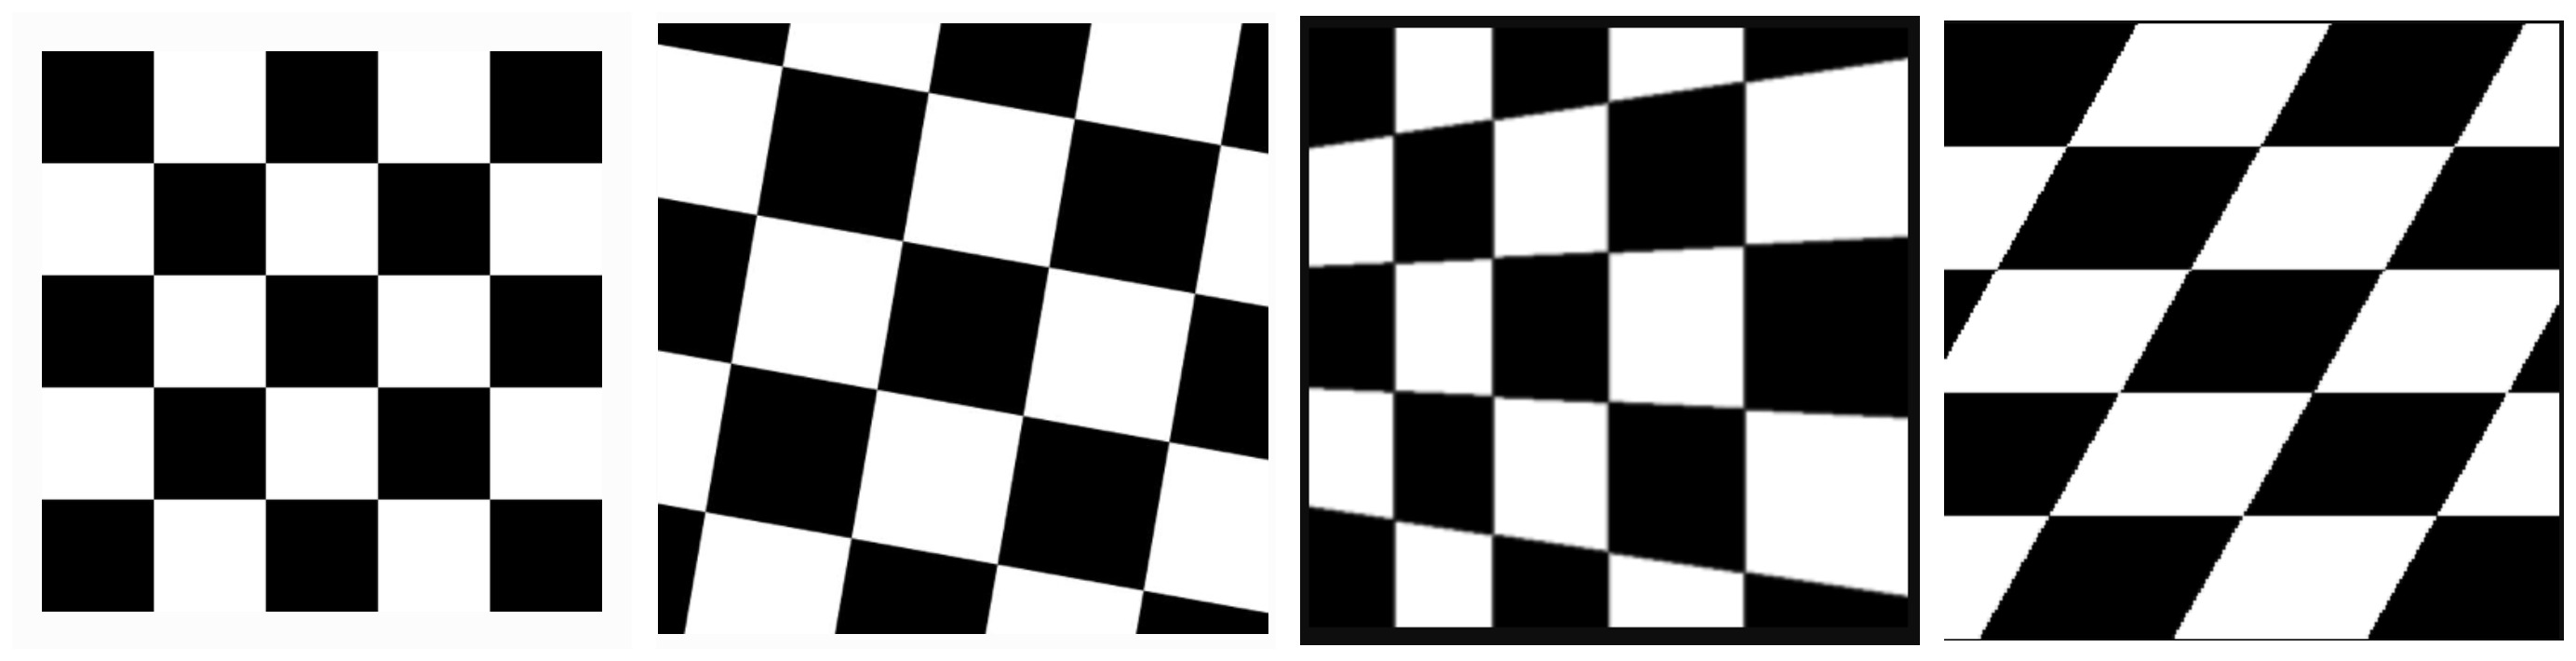
\includegraphics[width=1\textwidth]{fig/stroke_warping_transforamtions}
  \caption{An exmaple of rotation, skew, and shear (scale) transforamtions for stroke warping respectively from left to right \cite{stroke_warping_github_picture}}
\end{figure}


\section{Bayesian Approach}
\label{tit:bayesian-approach}
The astute reader should have noticed that, although quite different, all the introduced teqniques so far share a fundamental aspect. Precisely speaking, in all these teqniques, one obtains new training samples by applying a set of predefined random transformations on the annotated training data, and the augmentation procedure ends before the training phase starts. This widely used process is called the poor man's data augmentation (PMDA) \cite{poor_man_data_augmentation}. However, to the best of our knowledge, this is not the furthest that one can go. Indeed, the fact that neural networks are generally capable of learning complicated patterns and nonlinear relationships in images suggests that they should also be able to learn the latent variables so that they can enhance the data augmentation process dynamically.
In direct contrast to PMDA, in Bayesian data augmentation, the training set evolves dynamically and
in an iterative fashion during the training phase, which could considerably enhance the
generalization ability of a neural network. This approach uses class of teqniques to achieve this
matter as such as maximum a posterior probability (MAP) \cite{MAP_Bayesian} in Bayesian statistics and Generative
Adversarial Networks (GANs) . Before diving directly into technical details about the
Bayesian data augmentation, we need to briefly introduce generative models. Specifically, first, we
present the Generative Adversarial Networks (GANs) proposed initially by Goodfellow et al.
\cite{goodflew_bayesian_approach}. In what follow, we
will introduce GANs and after that and in the Bayesian approach description we will explain how this
approach uses the main idea of GANs and extend it to improve data augmentation.

\subsection{Generative Adversarial Networks (GANs)}
\label{tit:Generative-Adversarial-Network}
Generally, a Generative Adversarial Net is made up of two parts:
\begin{itemize}
\item{\textbf{Generator:}} As the name suggests, the generator in a GAN is responsible for generating new data and, at the same time, learns how to generate more plausible data. 
\item{\textbf{Discriminator:}} The discriminator portion of a GAN learns to distinguish real data from the synthetic data generated 
by the generator in the GAN and with this matter helps the generator to generate more plausible data.
\end{itemize}

Indeed, one can view the interaction between the generator and the discriminator of a GAN as a
minimax two-player game. Throughout the game, the generator's goal is to trick the discriminator
with synthetically generated data. The discriminator's goal, however, is to detect the model data
and to distinguish it from the real data. In the beginning, the discriminator may easily detect the
model data. However, after some iterations, the generator becomes sufficiently intelligent so that
it can produce synthetic data that is indistinguishable from the real data. Notice that, this means,
eventually, the discriminator's accuracy of classifying the real and fake data reduces to $50\%$,
where the classification is effectively random (predicts between $2$ classes
real or fake), and therefore the game is over. In some instances,
competition in this game enhances the generator's performance up to a point where detecting the
model data is impossible even for human eyes.
Technically speaking,  a GAN's task is to replicate a probability distribution.

The generator will be fed by random input \footnote{noise} to generate synthetic data. In general, GANs try to replicate a probability distribution. For this matter, they use loss function to measure the distance between the distribution of the generator's data and the distribution of the real data. As we mentioned Goodfellow el al. \cite{goodflew_bayesian_approach} suggest minimax loss in their work. The minimax loss defined as:

\begin{equation} \label{eq:minimax_loss}
  Minimax\ Loss = E_{x}[\log (D(x))]+E_{z}[\log (1-D(G(z)))]
\end{equation}


where $D(x)$  denotes the discriminator's estimate of the probability that real data instance x is
real and $D(G(z))$ denotes the discriminator's estimate of the probability that a fake instance is
real. It is clear that the Generator tries to minimize the (\ref{eq:minimax_loss}) and the
discriminator tries to maximize it. Figure \ref{fig:gan_architecture} shows a basic architecture of a
GAN.

\begin{figure}
  \centering
  \label{fig:gan_architecture}
  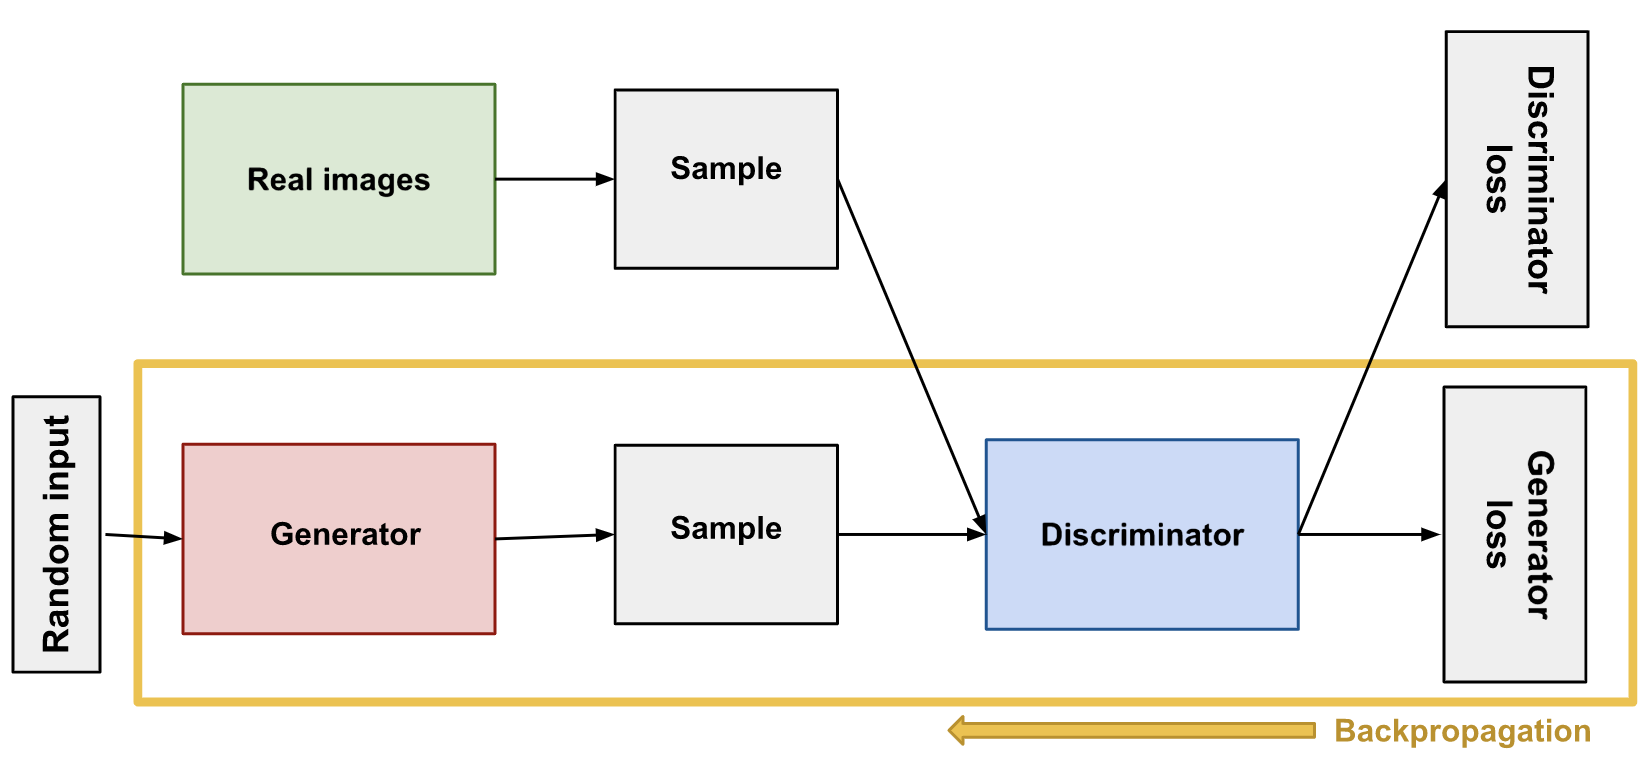
\includegraphics[width=1\textwidth]{fig/gan_architectur}
  \caption{GAN architecture
    \cite{google_bayesian_approach}}
\end{figure}

Now and after briefly introduction of GANs we can start with the \textbf{Bayesian Approach}. One of
the noteworthy work for data augmentation with the aid of the bayesian model proposed by Toan Tran
et al. \cite{refrence_bayesian_approach}. In this approach, our deep learning model tries to estimate the
distributions of labeled data and with aid of the estimated distributions optimizes the latent
variable used for data augmentation. The approach uses the GANs architecture skeleton to generate
synthetic data with the difference that the optimization of latent derived from the Bayesian model.
The principle idea for data augmentation using latent variables proposed by the statistical learning
community \cite{Statistical_data_augmentation}. Nevertheless applying the idea, directly into deep
learning seeks a massive computational effort. Therefore we talked before about the estimation. To
be more precise, the
approach uses a novel Bayesian data augmenation algorithm, called Generalized Monte Carlo Expectation Maximization
(GMCEM). This algorithm augments training data and mutually optimizes the network parameters. The
algorithm successively generates synthetic data and use Monte Carlo to estimate the expected value
of the network parameters given the previous estimate instead of calculating loss function. After
the estimation of the expected value, the parameter values will be updated with stochastic gradient
descent (SGD). In the end, the algorithm and approach turned in to reality with the aid of GANs. The
proposed GAN consists of one generator and $2$ discriminators. As we in the GANs section
(\ref{tit:Generative-Adversarial-Network}) discussed the generator is responsible to generate
synthetic data and one of our discriminators distinguishes fake and real data. However, the second
discriminator discriminates between the classes of data. Figure
\ref{fig:bayesian-approach-gan-architecture} represents the utilized netwok architecture in this
approach visually. This proposed architecture is nearly similar to the Auxiliary classifier GANs
(AC-GANs) \cite{AC-GANS}. Nevertheless, in the AC-GANs discriminator responsible for both
classification real-or-fake data and data labels (classes) and in our network we utilized $2$
discriminators separately for this matter.

\begin{figure}
  \centering
  \label{fig:bayesian-approach-gan-architecture}
  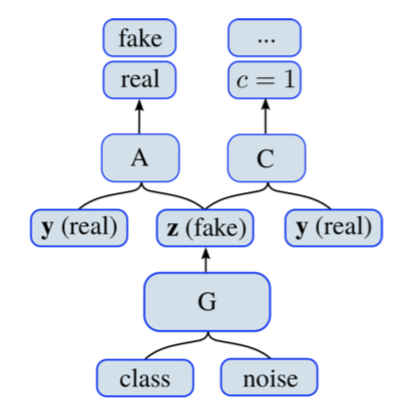
\includegraphics[width=0.5\textwidth]{fig/bayesian-approach-gan-architecture}
  \caption{The network architecture of Bayesian data augmentaion approch \cite{refrence_bayesian_approach}. G: Generator, A: Authenticator, C: Classifier.}
\end{figure}

In the following, we will explain the utilized algorithm formally from the Toan Tran el al. work \cite{refrence_bayesian_approach}. As we mentioned the goal is to estimate the parameters of the neural networks using labeled data. The training process is defined by the following optimization problem:

\begin{equation} \label{eq:optimization-problem}
  \theta^{*}=\arg \max \log p(\theta | \mathbf{y})
\end{equation}
Where training set denoted as $\mathcal{Y}=\left\{\mathbf{y}_{n}\right\}_{n=1}^{N}$ with $y=(t,x)$
and $t\in\{1, ..., K\}$ (Classes-Set) and data samples $\mathbb{R}^D$ and $\theta$ denoted as
model (network) parameters and observed posterior defined as:
\begin{equation} \label{eq:observed-posterior}
  p(\theta | \mathbf{y})=p(\theta | t, \mathbf{x}) \propto p(t | \mathbf{x}, \theta) p(\mathbf{x} | \theta) p(\theta)
\end{equation}
Now if we assume that the data samples $\mathcal{Y}$ are conditionaly independent, we can define the
following loss function which maximize the (\ref{eq:optimization-problem}).

\begin{equation} \label{eq:loss-function}
  \log p(\theta | \mathbf{y}) \approx \log p(\theta)+\frac{1}{N} \sum_{l}^{N}\left(\log p\left(t_{n} | \mathbf{x}_{n}, \theta\right)+\log p\left(\mathbf{x}_{n} | \theta\right)\right)
\end{equation}
where $p(\theta)$ denotes a prior on the distribution of the deep learning model parameters, $p(t_n|x_n, \theta)$
represents the conditional likelihood of label $t_n$, and $p(x_n|\theta)$ is the likelihood of the
data $x$.

After estimation and optimization the $\theta$ on our training set, it is the time to generate
synthetic data from $y$ using latent variable $z$. Therefore the augmented $p(\theta | y,z)$ can be
estimated. The latent variable $z$ as same as $y$ defined as $z = (t^{\alpha}, x^{\alpha})$ where
$t^{\alpha} \in \{1,...,K\}$ denotes associated label and $x^{\alpha} \in   \mathbb{R}^D$ is
synthesized sample. As we mentioned to avoid a heavy and most likely interminable computation,
instead of the Expectation-Maximization (EM) algorithm we will use Generalized Monte Carlo EM
Algorithm to estimate the expected value and maximize it.Hence the augmented posterior $p(\theta|y,
  z)$ for latent variable $z$ will be as follow:

\begin{equation} \label{eq:latent-variable}
  p(\theta | \mathbf{y}, \mathbf{z})=\frac{p(\mathbf{y}, \mathbf{z}, \theta)}{p(\mathbf{y}, \mathbf{z})}=\frac{p(\mathbf{z} | \mathbf{y}, \theta) p(\theta | \mathbf{y}) p(\mathbf{y})}{p(\mathbf{z} | \mathbf{y}) p(\mathbf{y})}=\frac{p(\mathbf{z} | \mathbf{y}, \theta) p(\theta | \mathbf{y})}{p(\mathbf{z} | \mathbf{y})}
\end{equation}
where the expectation step will be defined as follow:
\begin{equation} \label{eq:expectation-latent-variable}
  p(\theta | \mathbf{y}, \mathbf{z})=\frac{p(\mathbf{y}, \mathbf{z}, \theta)}{p(\mathbf{y}, \mathbf{z})}=\frac{p(\mathbf{z} | \mathbf{y}, \theta) p(\theta | \mathbf{y}) p(\mathbf{y})}{p(\mathbf{z} | \mathbf{y}) p(\mathbf{y})}=\frac{p(\mathbf{z} | \mathbf{y}, \theta) p(\theta | \mathbf{y})}{p(\mathbf{z} | \mathbf{y})}
\end{equation}
where \(\mathbf{z}_{m} \sim p\left(\mathbf{z} | \mathbf{y}, \theta^{i}\right),\) for \(m \in\{1,
\ldots, M\} .\) In \((6),\) if the label \(t_{m}^{a}\) of the \(m^{t h}\) synthesized sample
\(\mathbf{z}_{\mathbf{m}}\) is known, then \(\mathbf{x}_{m}^{a}\) can be sampled from the
distribution \(p\left(\mathbf{x}_{m}^{a} | \theta, \mathbf{y}, t_{m}^{a}\right) .\) Hence, the
conditional distribution \(p(\mathbf{z} | \mathbf{y}, \theta)\) can be decomposed as:

\begin{equation}
  p(\mathbf{z} | \mathbf{y}, \theta)=p\left(t^{a}, \mathbf{x}^{a} | \mathbf{y}, \theta\right)=p\left(t^{a} | \mathbf{x}^{a}, \mathbf{y}, \theta\right) p\left(\mathbf{x}^{a} | \mathbf{y}, \theta\right)
\end{equation}
where \(\left(t^{a}, \mathbf{x}^{a}\right)\) are conditionally independent of y given that all the
information from the training set y is summarized in \(\theta\) this means that \(p\left(t^{a} |
\mathbf{x}^{a}, \mathbf{y}, \theta\right)=p\left(t^{a} | \mathbf{x}^{a}, \theta\right),\) and
\(p\left(\mathbf{x}^{a} | \mathbf{y}, \theta\right)=p\left(\mathbf{x}^{a} | \theta\right)\).
Now with respect to the $\theta$ for the maximization step with concern of removing the independent terms
for $\theta$ will derived the maximization of $\hat{Q}\left(\theta, \theta^{i}\right)$ as follow:

\begin{equation}
  \begin{aligned}
     & \hat{Q}\left(\theta, \theta^{i}\right)=\log p(\theta)+\frac{1}{N} \sum_{n=1}^{N}\left(\log p\left(t_{n} | \mathbf{x}_{n}, \theta\right)+\log p\left(\mathbf{x}_{n} | \theta\right)\right)+\frac{1}{M} \sum_{m=1}^{m} \log p\left(\mathbf{z}_{m} | \mathbf{y}, \theta\right) \\
     & =                                                                                                                                                                                                                                                                           \\
     & \log p(\theta)+\frac{1}{N} \sum_{n=1}^{N}\left(\log p\left(t_{n} | \mathbf{x}_{n}, \theta\right)+\log p\left(\mathbf{x}_{n} | \theta\right)\right)+\frac{1}{M}
    \sum_{m=1}^{n}\left(\log p\left(t_{m}^{a} | \mathbf{x}_{m}^{a}, \theta\right)+\log p\left(\mathbf{x}_{m}^{a} | \theta\right)\right)
  \end{aligned}
\end{equation}

After all, we estimate the $\theta^{i +1}$ so that $\hat{Q}(\theta^{i +1}, \theta^{i}) >
\hat{Q}(\theta^{i}, \theta^{i})$. To reduce the computation complexity as we mentioned instead of
gradient descent, stochastic gradient decent (SGD) utilized for estimating the $\theta^{i +1}$. The
iteration will be continued until $|\theta^{i +1} - \theta^{i}|$ get sufficiently small. 

As we made it clear, the above formal explanations and equations are derived from \cite{refrence_bayesian_approach} and in some points are matched one-to-one.  

%\section{Manifold Approach}
%\label{tit:manifold-approach}

\chapter{Pragmatic Expriments}
in this Chapter 

\section{CNNs Architecture}
In this section, we will introduce our classifiers (CNNs) architecture for various datasets which we
introduced in the chapter (\ref{tit:data-representation}). We picked our CNNs architecture from
different sources regarding their non-heavy complexity and desirable accuracy.  Maybe our chosen
CNNs architecture doesn't provide the best-reported accuracy on datasets, but while we use the
same CNN-architecture for each dataset and we aim to compare various data augmentation approaches on
each dataset, it would not affect our results. Moreover, as we will report in chapter (\ref{tit:results})
our result are not so far away from best-reported accuracy on the orginal dataset.

\subsection{MNIST}
For the MNIST dataset, we have chosen a semi-simple CNN architecture from \cite{MNIST_CNN_Architecture} with $2$
convolutional layers and $2$ fully connected layers. ReLU function is utilized as the activation
function. For training and to calculate the loss function, \textbf{CrossEntropyLoss} and
to optimize the network's parameters \textbf{Adam optimizer} \cite{adam-optimizer} from the Pytorch have been
chosen. The learning rate for Adam optimizer is set to $0.001$. To reduce overfitting, a
drop-out layer is placed at the end of the second convolutional layer. Figure \ref{fig:MNIST_CNN_Architecture} represents the explained CNN architecture visually.

\begin{figure}
  \centering
  \label{fig:MNIST_CNN_Architecture}
  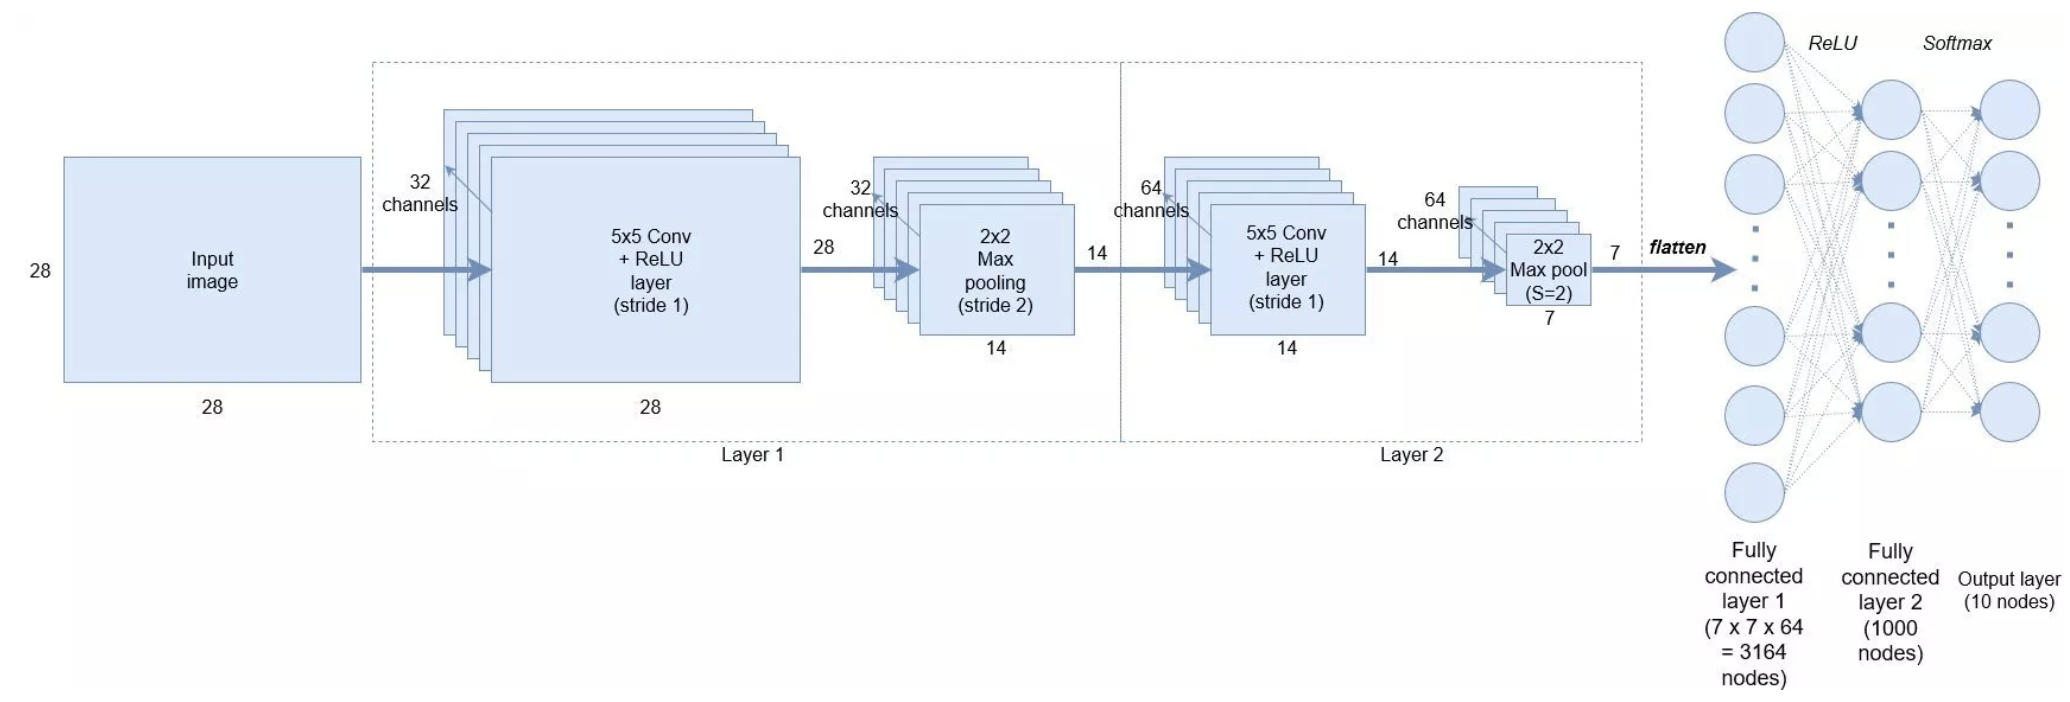
\includegraphics[width=1\textwidth]{fig/MNIST-CNN-Architecture}
  \caption{CNN Architecture for training the MNIST dataset \cite{MNIST_CNN_Architecture_Image}}
\end{figure}


\subsection{Fashsion-MNIST}
The Fashion-MNIST dataset use CNN architectur deriven form \cite{TODO} with $2$
convolutional layers and $2$ fully connected layers as same as MNIST dataset just with this
different of up- and downsampling and kernels sizes. ReLU function is utilized as the activation
function. The learning rate for Adam optimizer is set to $0.001$. Figure \ref{fig:Fashion_MNIST_CNN_Architecture} represents the explained CNN architecture visually.

\begin{figure}
  \centering
  \label{fig:Fashion_MNIST_CNN_Architecture}
  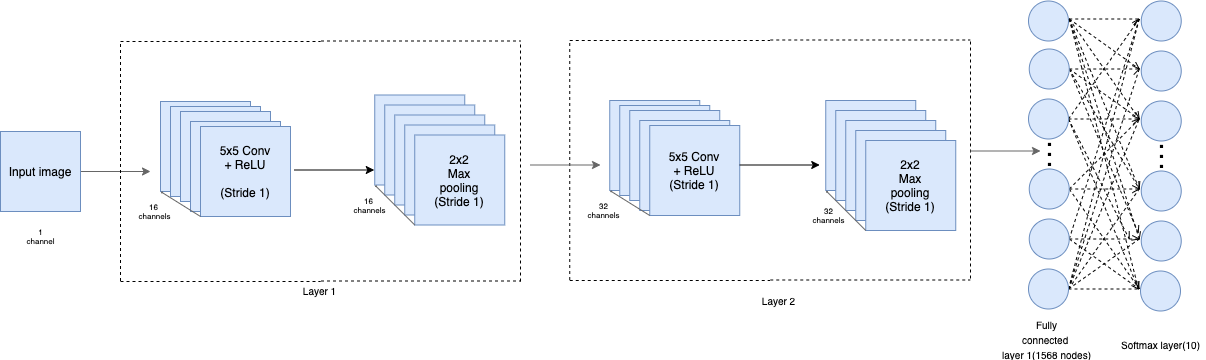
\includegraphics[width=1\textwidth]{fig/Fashion-MNIST-CNN-Architecture}
  \caption{CNN Architecture for training the Fashion-MNIST dataset}
\end{figure}

\subsection{CIFAR-10}
For the CIFAR-10 dataset, we have chosen a bit more complex CNN architecture from \cite{CIFAR_CNN_Architecture} with $6$
convolutional layers and $3$ fully connected layers. ReLU function is utilized as the activation
function. For training and to calculate the loss function, \textbf{CrossEntropyLoss} and
to optimize the network's parameters \textbf{Adam optimizer} as same as $2$ previous CNNs architecture have been
chosen. The learning rate for Adam optimizer is set again to $0.001$. To reduce overfitting, a
drop-out layer is placed at the end of the fourth convolutional layer. Figure \ref{fig:CIFAR_CNN_Architecture} represents the explained CNN architecture visually. 


\begin{figure}
  \centering
  \label{fig:CIFAR_CNN_Architecture}
  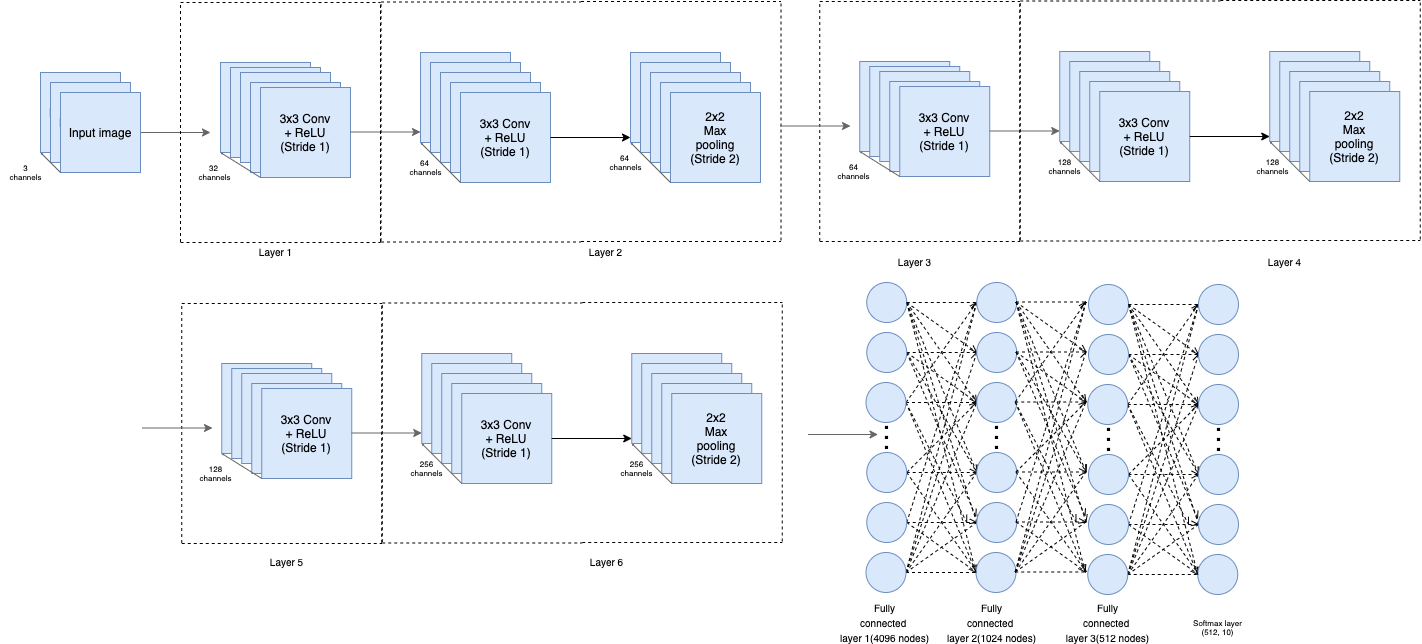
\includegraphics[width=1\textwidth]{fig/CIFAR-CNN-Architecture}
  \caption{CNN Architecture for training the CIFAR-10 dataset}
\end{figure}

\section{Implementaions}
In what follow, we will point out shortened to the manner of proceed and implementation of each
approach and technique. 

In general to put the idea of label preserving transformations and their techniques
into practice, we utilized an external library in Python for data augmentation called Augmentor \footnote{\url{https://github.com/mdbloice/Augmentor}}. As
we mentioned the main part (Machine Learning) carried out with a powerful library form Facebook
called Pytorch \footnote{\url{https://pytorch.org/}}. 

\subsection{Image Translations}
\subsection{Elastic Distortion}
\subsection{Stroke Warping}
\subsection{Bayesian Approach}


\chapter{Result \& Comparison}
\label{tit:results}
In this chapter, we will publish the results of our pragmatic experiments on each introduced
approach and dataset and following that we will discuss and compare the advantage and disadvantages
of each approach and their behavior on different datasets. These results and comparisons do not only
provide a good insight into each approach but also is a preface of the next chapter and the manner
of genesis the idea of new approaches. 

To have a good and comprehensive comparison, we tried the approaches and techniques in different
environments. To be more precise, we considered the accuracy of the original datasets (with all
train and test samples) and accuracy of learning without augmentation on the few-shot dataset to
keep tracking of the differences between accuracy of them with augmentation on the few-shot dataset.
Due to the comprehensive comparison, we tried various of the k-shot datasets: 

\begin{equation}
  k=
  \begin{cases}
    \{1, 5, 10\}  & \text{if}\ dataset= 
    \ MNIST \ or \ Fashion-MNIST \\
    \{10, 20, 30\} & \text{if}\ dataset= \ CIFAR-10
  \end{cases}
\end{equation}

Additionally, to compare the result in fair circumstances we augmented the data by factor 100 (100X)
for the training and by factor 10 (10X) with each augmentation technique. In the end and to provide
a more realistic result we used 10-fold cross validation \cite{cross_validation}. That means for each k-shot learning, we
derived 10 different and random k-shot datasets to calculate more realistic accuracy for each
technique.

The figures \ref{fig:MNIST_result}, \ref{fig:Fashion_MNIST_result}, and
\ref{fig:CIFAR_10_result} represent these results and accuracy for each approach and technique
respectively for
MNIST, Fashion-MNIST, and CIFAR-10 datasets.


\begin{figure}
  \centering
  \label{fig:MNIST_result}
  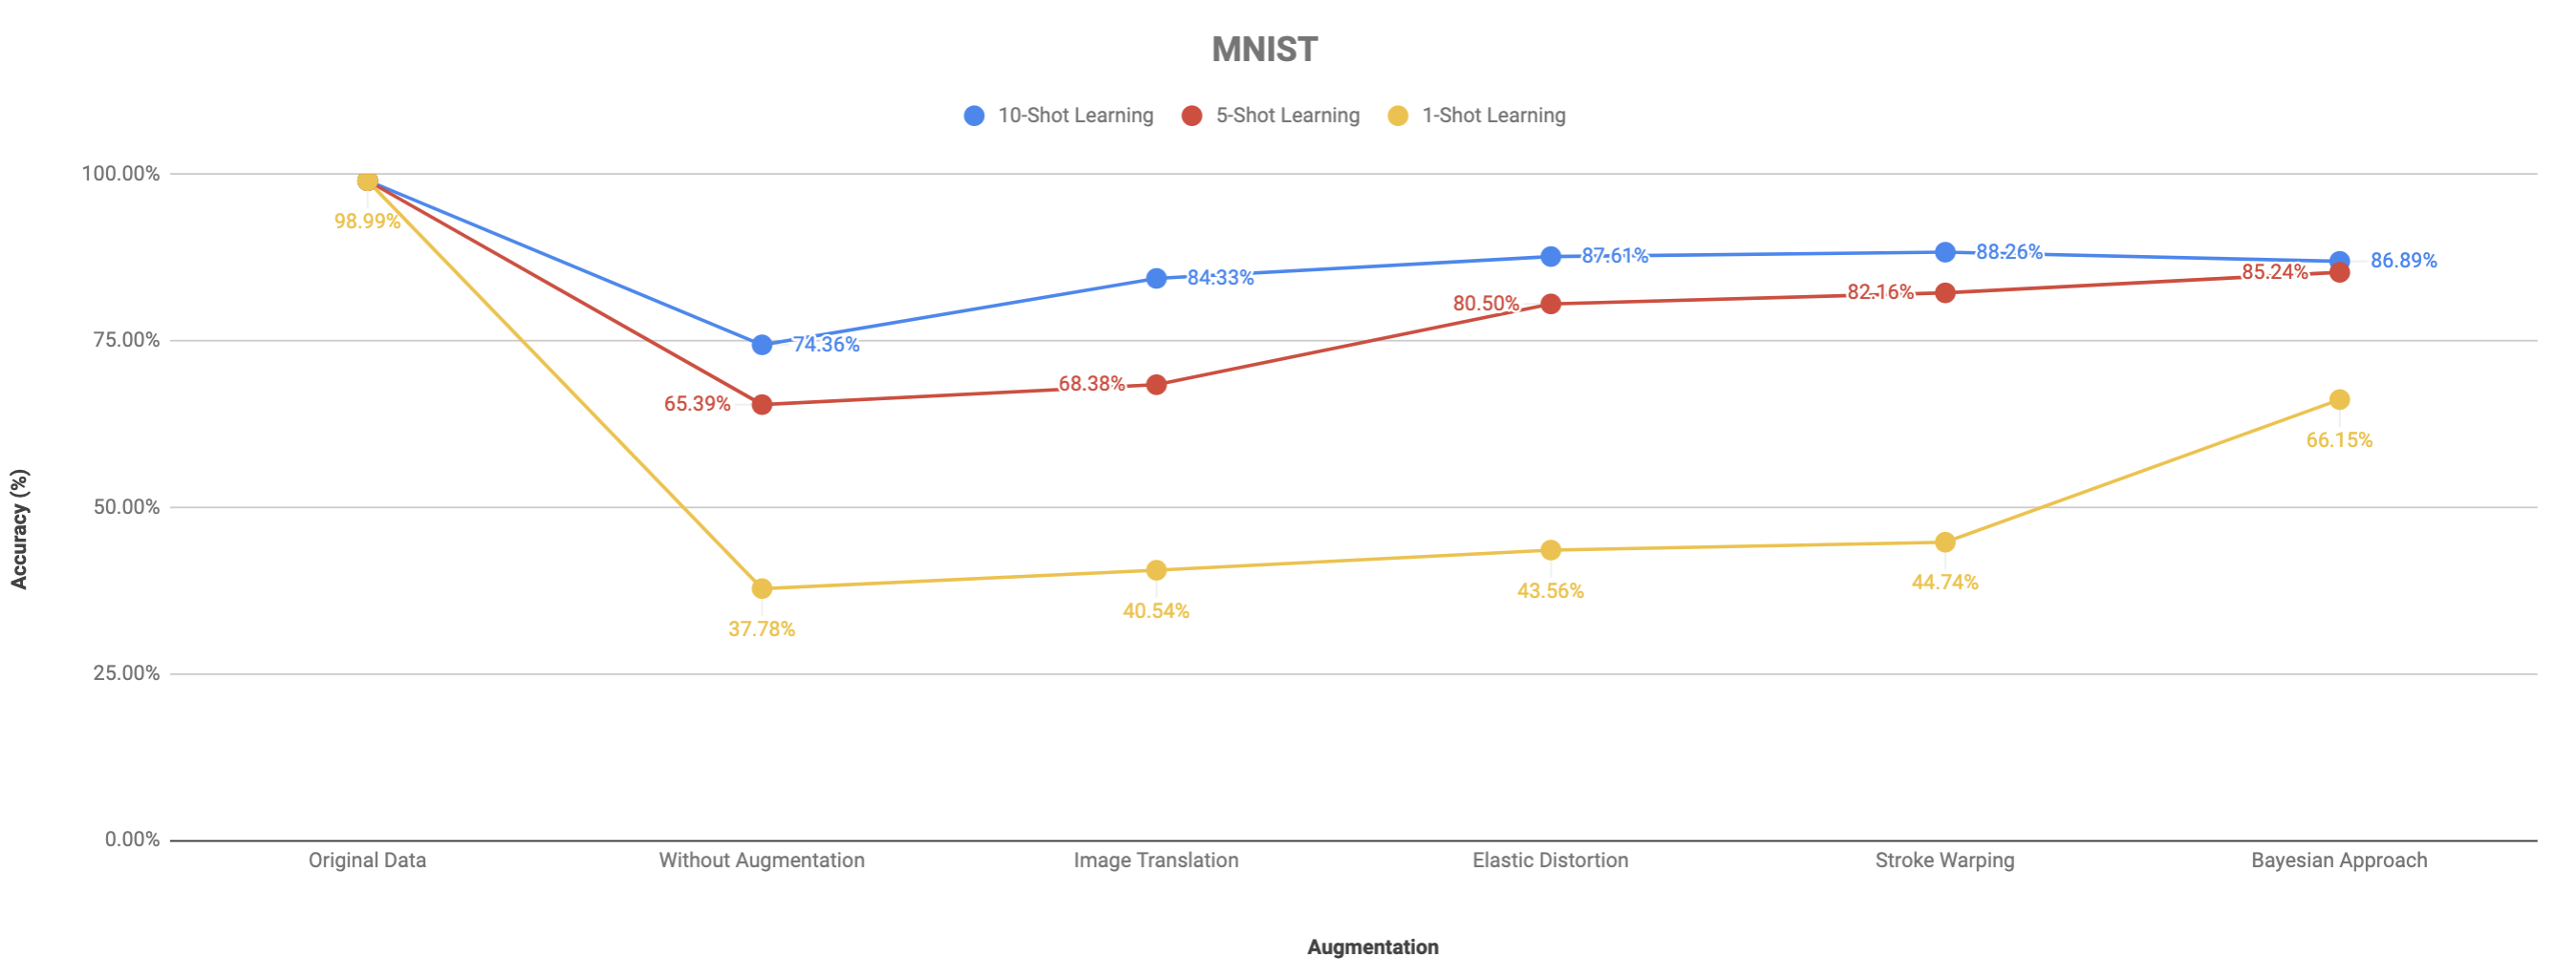
\includegraphics[width=1\textwidth]{fig/result/mnist-result}
  \caption{Result of augmentation techniques on MNIST dataset}
\end{figure}


\begin{figure}
  \centering
  \label{fig:Fashion_MNIST_result}
  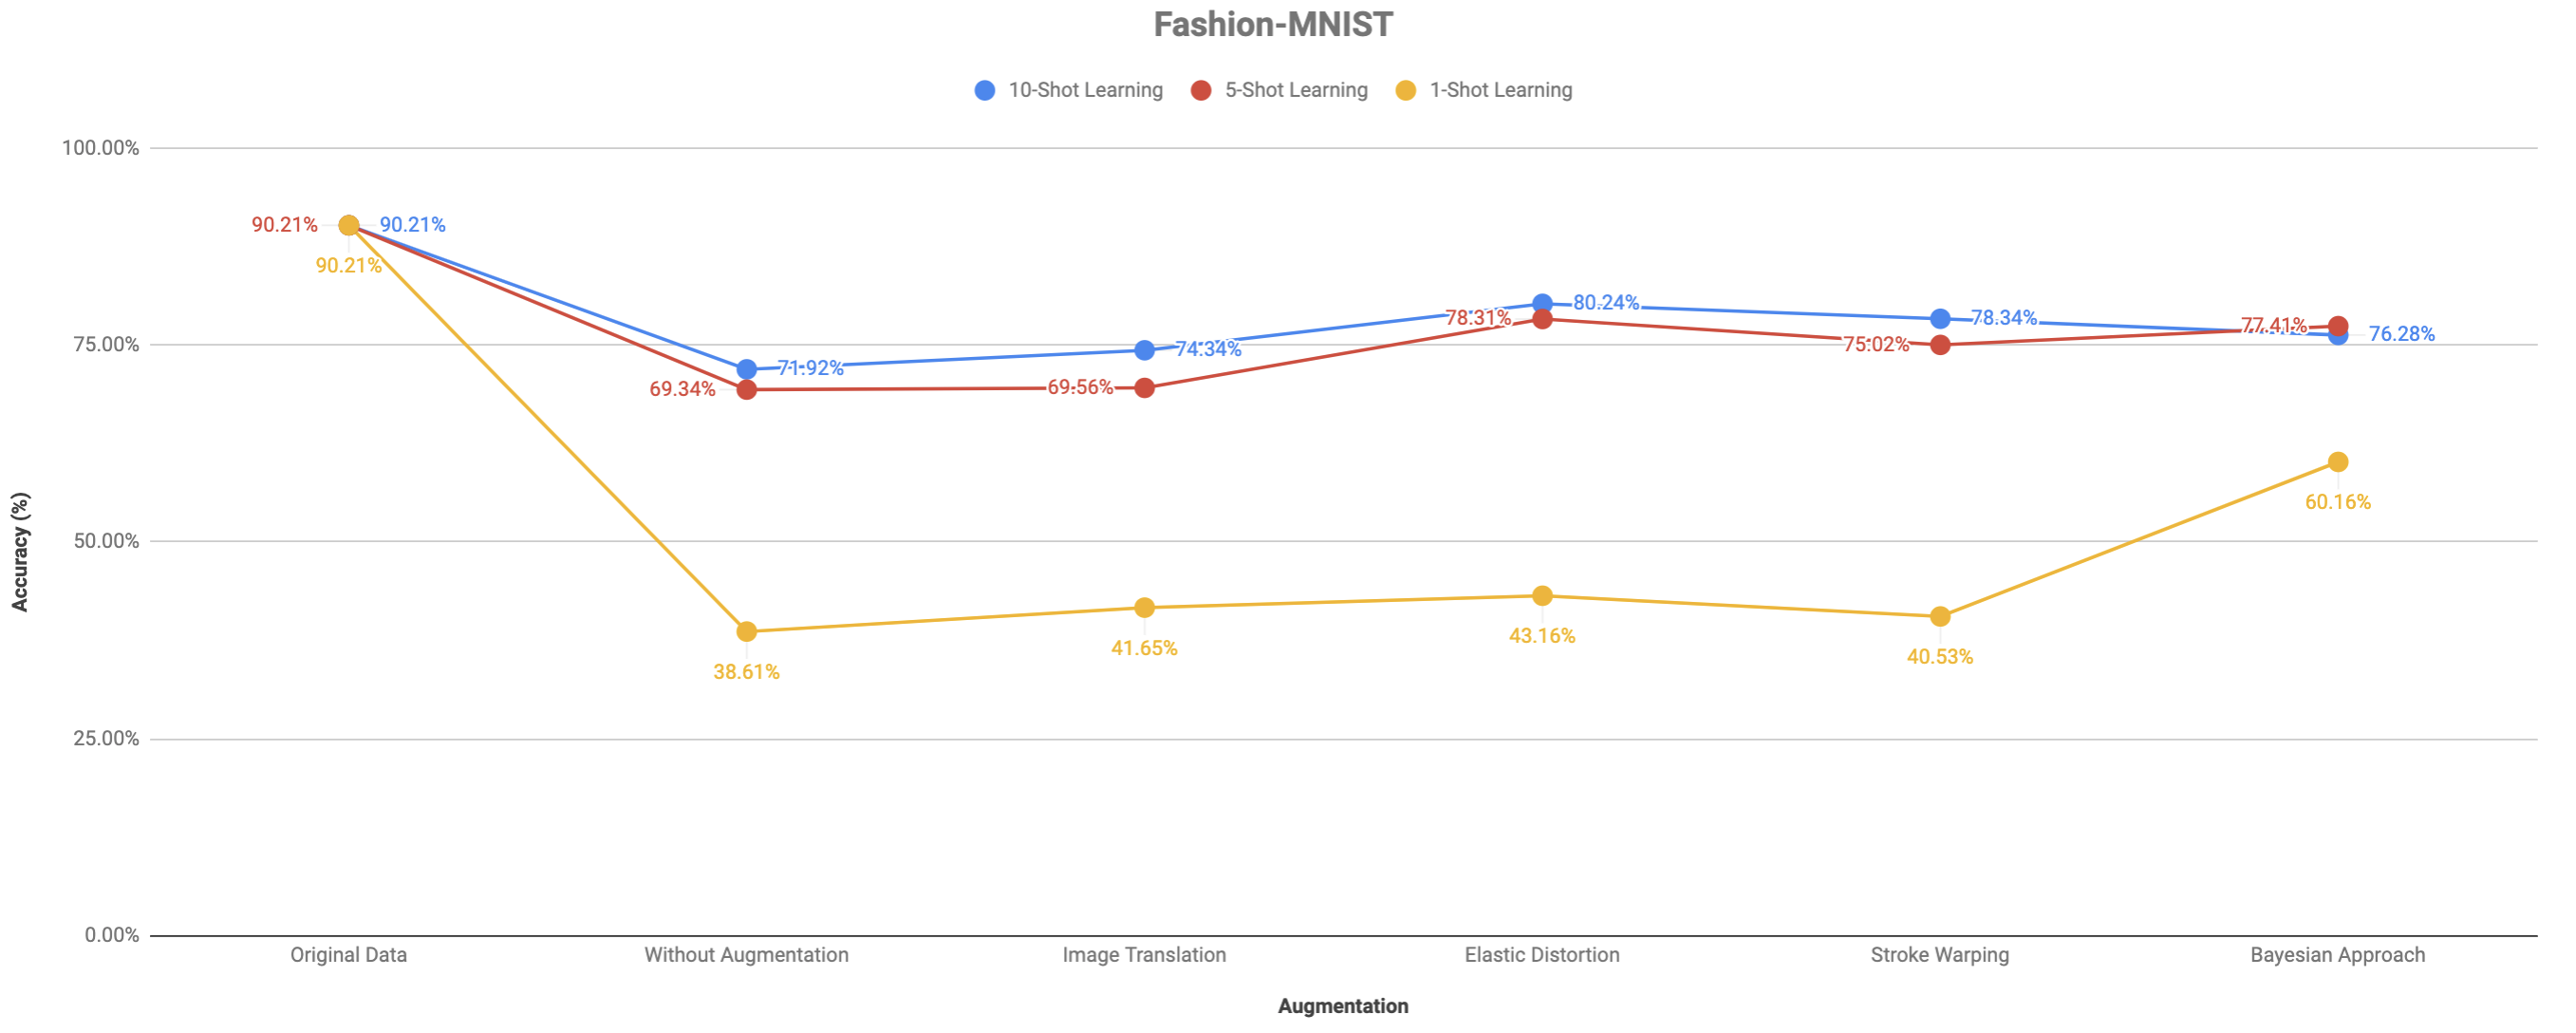
\includegraphics[width=1\textwidth]{fig/result/fashion-mnist-result}
  \caption{Result of augmentation techniques on Fashion-MNIST dataset}
\end{figure}


\begin{figure}
  \centering
  \label{fig:CIFAR_10_result}
  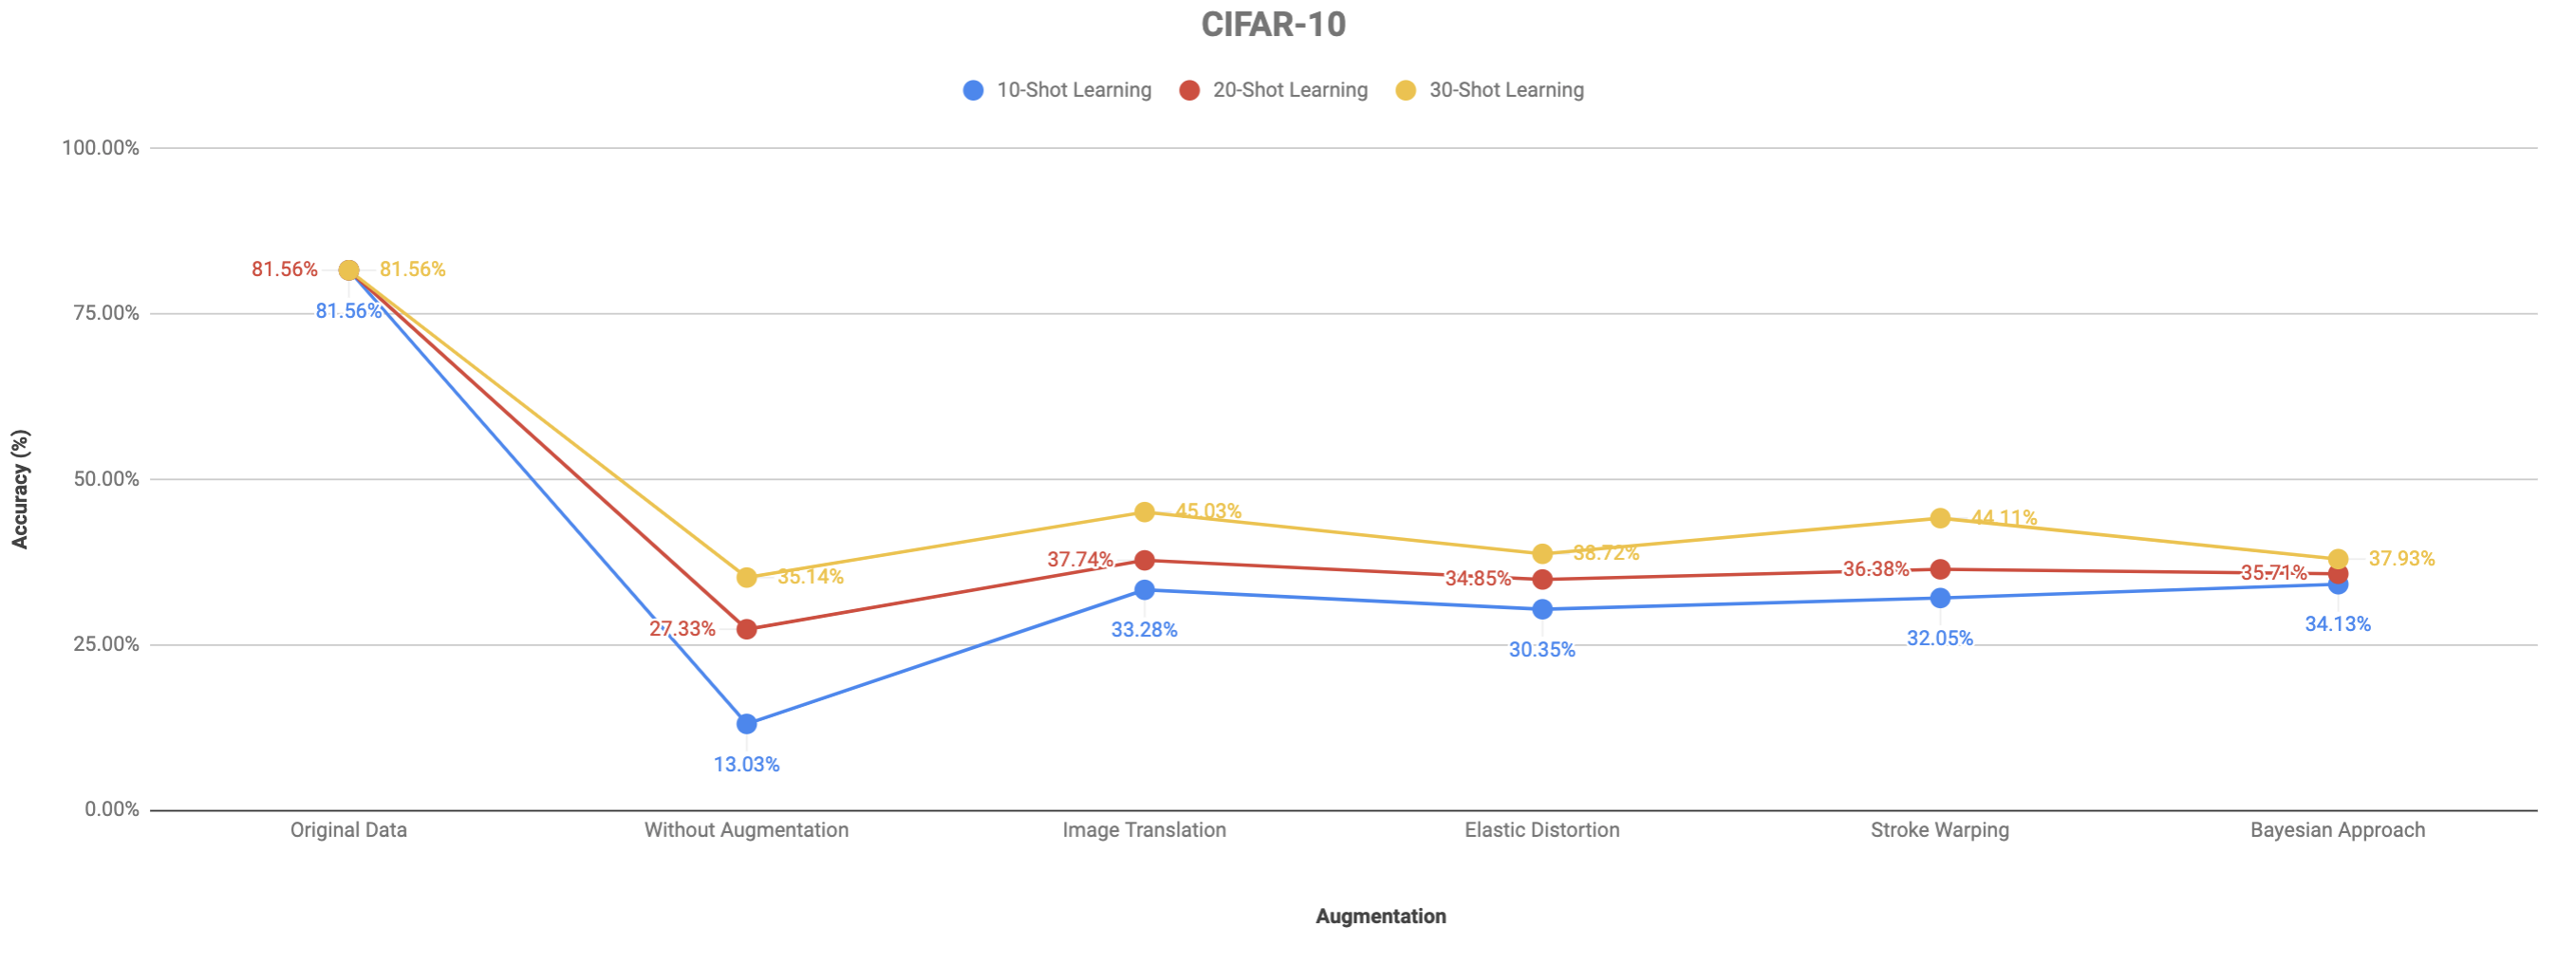
\includegraphics[width=1\textwidth]{fig/result/cifar-10-result}
  \caption{Result of augmentation techniques on CIFAR-10 dataset}
\end{figure}

The first look to the figures \ref{fig:MNIST_result} and \ref{fig:Fashion_MNIST_result} expose, that there is
a significant gap between the accuracy of 10 and 5-shot learning and 1-shot learning without augmentation. Besides,
it shows that k-shot learning is not linearly correlated with accuracy for each technique. As there is
just one sample for each class, the CNN involves pretty soon with overfitting. Nevertheless, the
accuracy is about $30\%$ and that means that the prediction is not randomly even for 1-shot
learning on MNIST and Fashion-MNIST. 

Another impression of the first look to the figure \ref{fig:CIFAR_10_result} is the considerable gap between accuracy on original data and few-shot learning on CIFAR-10. This matter exposes the major role of color (RGB images) in learning and accuracy. As long as this gap is not observable on MNIST and Fashion-MNIST. 

\chapter{Contribution Of Work}